%!TEX root = main.tex
%%%%%%%%%%%%%%%%%%%%%%%%%%%%%%%%%%%%%%%%%%%%%%%%%%%


% ========================================
\section{Numerical experiments}\label{sec:Num-Exp}
% ========================================
%
We present numerical results of Monte Carlo, multilevel Monte Carlo, and multi-fidelity Monte Carlo  methods for estimating $\mathbb{E}(u)$ in the Grad-Shafranov free boundary problem. The extending multilevel methodology is detailed in \cite{ElLiSa:2023,Gi:2008,Gi:2015}. The nonlinear system \eqref{eq:FreeBoundary_GS} uses source profiles $p(\psi)$ and $g(\psi)$ from \eqref{eq:source} with fixed parameters
%
\begin{equation}\label{eq:CentralParameterValue}
r_0=6.2m,\,\,\beta=0.5978, \,\, \alpha_1 = 2, \,\,  \alpha_2=1.395, \,\, j_0=1.3655 \times 10^6 A/m^2,\,\,  \mu_0=1.2566\times 10^{-6} N/A^2.
\end{equation}
%
The computational setup adopts the ITER tokamak geometry \cite{Amoskov:2009} following \cite{FaHe:2017}. The system comprises twelve magnetic coils with \textit{reference currents} $\boldsymbol{I} = (I_1,\dots,I_{12})$ specified as
%
\begin{equation}\label{eq:CentralCurrentValue}
{\renewcommand{\arraycolsep}{2pt}
\begin{array}{llll}
I_1 = -1.4 \times 10^{6}A, \quad & I_2 = -9.5 \times 10^{6}A, \quad & I_3 = -2.0388 \times 10^{7}A, \quad & I_4 = -2.0388 \times 10^{7}A, \\
I_5 = -9 \times 10^{6}A, \quad & I_6 = 3.564 \times 10^{6}A, \quad & I_7 = 5.469 \times 10^{6}A, \quad & I_8 = -2.266 \times 10^{6}A, \\
I_9 = -6.426 \times 10^{6}A, \quad & I_{10} = -4.82 \times 10^{6}A, \quad & I_{11} = -7.504 \times 10^{6}A, \quad & I_{12} = 1.724 \times 10^{7}A.
\end{array}
}
\end{equation}
%
Parametric uncertainty is modeled via independent uniformly distributed perturbations of magnitude $\tau = 2\%$ around these reference values.


For MFMC implementation, we construct a hierarchy of low-fidelity surrogate models using level-1 sparse grid stochastic collocation on six non-nested meshes $\{\mathcal{T}_\ell\}_{\ell=0}^5$. These meshes are generated through geometry-conforming uniform refinement of an ITER base configuration (30,449 nodes), preserving critical geometric fidelity via curvature-adaptive discretization essential for accurate plasma boundary resolution. The resulting computational hierarchy spans from $2.6\times 10^3$ to $1.4\times 10^6$ degrees of freedom (Table~\ref{Tab:MFMC_parameters}). The high-fidelity solver, implemented in \texttt{FEEQS.m} \cite{Heumann:feeqsm} and algorithmically grounded in \texttt{CEDRES++} \cite{FaHe:2017,CEDRES}, discretizes the weak formulation of \eqref{eq:FreeBoundary} using piecewise linear finite elements and resolves the inherent nonlinearity via a globalized Newton method. This computationally intensive approach constitutes our \textit{direct solver}, providing benchmark solutions against which multifidelity approximations are evaluated.


Error control for the MC, MLMC, and MFMC estimators is governed by the mean square error decomposition with balanced allocation between discretization and sampling errors ($\theta = 0.5$). For tolerances $\epsilon \in \{2,4,6,8,10,20,40,80\} \times 10^{-4}$ -- all exceeding the finest mesh discretization error -- we determine minimal discretization levels $L$ such that the discretization error remains below $\theta \epsilon^2$, yielding $L = 5,4,4,4,4,3,3,2 $ respectively. The high-fidelity model is consequently defined on $\mathcal{T}_L$ at each tolerance level. All computational workflows are executed in MATLAB R2024a on Rice University's NOTSx HPC cluster.



% The system consists of 298 dual-socket compute blades housed across HPE s6500, HPE Apollo 2000, and Dell PowerEdge C6400 chassis. All nodes are interconnected via a high-speed network with 10 or 25 Gigabit Ethernet.



% =============================
\subsection{Welford's algorithm}
% =============================
Welford's algorithm \cite{Welford:1962} provides a numerically stable framework for incremental computation of sample statistics with $\mathcal{O}(1)$ memory complexity, essential for large-scale multifidelity simulations where full sample retention is infeasible. For models $k \in \{1, \dots, K\}$ with $k=1$ denoting the high-fidelity model, we initialize accumulators $m_k^{(0)} = 0$ (mean), $v_k^{(0)} = 0$ (unnormalized variance), and $r_k^{(0)} = 0$ (unnormalized covariance for $k \geq 2$). At each sample iteration $i \geq 1$, given sample $\boldsymbol{\omega}^{(i)}$, the algorithm computes outputs $u_k^{(i)}$ and executes updates
%
\begin{align*}
    &m_k^{(i)} = m_k^{(i-1)} + \frac{1}{i}\left( u_{k}^{(i)}-m_k^{(i-1)}\right),\qquad v_k^{(i)} = v_k^{(i-1)} + \left\langle  u_{k}^{(i)}-m_k^{(i-1)}, \;\; u_{k}^{(i)}-m_k^{(i)}\right\rangle_U,\\
    &r_k^{(i)} = r_k^{(i-1)} + \left \langle  u_{1}^{(i)}-m_{1}^{(i-1)},\;\; u_{k}^{(i)}- m_{k}^{(i)}\right\rangle_U, \quad \text{for }\;\; k\ge 2.
\end{align*}
%
After processing $N$ samples, final statistics are computed as $\widehat{\mu}_k = m_k^{(N)}$, $\widehat{\sigma}_k^2 = v_k^{(N)}/(N-1)$, and $\widehat{\text{Cov}}_{1,k} = r_k^{(N)}/(N-1)$, with correlations $\widehat{\rho}_{1,k} = \widehat{\text{Cov}}_{1,k}/(\widehat{\sigma}_1 \widehat{\sigma}_k)$. These yield unbiased estimators for means, variances and covariances. The algorithm's stability stems from orthogonal residual updates that minimize rounding error propagation, particularly critical when estimating correlations near $\pm 1$ $(\widehat{\text{Cov}}_{1,k}\approx \widehat\sigma_1\widehat\sigma_k)$ where conventional methods falter.

% From these updates, the sample standard deviations of the high- and low-fidelity models and the covariance are computed as 
% $\sigma_k^{(i)} = \sqrt{v_k^{(i)}/(i-1)},\;\text{Cov}^{(i)} = r_k^{(i)}/(i-1).$
% %
% \[
% \sigma_H^{(i)} = \sqrt{v_H^{(i)}/(i-1)},\quad \sigma_L^{(i)} = \sqrt{ v_L^{(i)}/(i-1)},\quad \text{Cov}^{(i)} = r^{(i)}/(i-1).
% \]
% %
% These are unbiased estimators, satisfying 
% $\mathbb{E}[m_k^{(N)}]=\mu_k,\; \mathbb{E}[\sigma_k^{(N)}]=\sqrt{\mathbb{E}[v_k^{(N)}]/(N-1)}=\sigma_k, \;\mathbb{E}[\text{Cov}^{(N)}] = \mathbb{E}[r_k^{(N)}]/(N-1) = \rho_{1,k}\sigma_1\sigma_k$.
% %
% \begin{align*}
%     \mathbb{E}\left[m_H^{(N)}\right]&=\mu_1,\quad \mathbb{E}\left[ m_L^{(N)}\right]=\mu_k, \\
%     % \quad \mathbb{E}(v_w^{(N)})=(N-1)\sigma_1^2, \quad\mathbb{E}(\widehat v_w^{(N)})=(N-1)\sigma_k^2, \\
%     \mathbb{E}\left[\sigma_H^{(N)}\right]&=\sqrt{\mathbb{E}\left[v_H^{(N)}\right]/(N-1)}=\sigma_1, \quad \mathbb{E}\left[\sigma_L^{(N)}\right]=\sigma_k, \quad\mathbb{E}\left[\text{Cov}^{(N)}\right] = \frac{\mathbb{E}\left[r^{(N)}\right]}{N-1} = \rho_{1,k}\sigma_1\sigma_k.
% \end{align*}
% %




% =============================
\subsection{Offline cost of surrogate construction and parameter estimation in MFMC}
% =============================
The offline computational expenditure in MFMC decomposes into surrogate model construction and statistical parameter estimation. For surrogate modeling, we use level $q=1$ sparse grid stochastic collocation as detailed in Section~\ref{sec:SC} to build low-fidelity models on spatial grid levels $0$ through $L-1$, where $L$ denotes the high-fidelity grid level satisfying the prescribed discretization error tolerance $\epsilon$. Table~\ref{Tab:Offline_cost} quantifies the exponential growth in surrogate construction time across tolerance values $\epsilon \in [2\times 10^{-4}, 8\times 10^{-3}]$, corresponding to refinement levels $L = 2$ to $5$.
%
\begin{table}[ht]
\centering
\scalebox{1.0}{
\begin{tabular}{|c|c|c|c|c|}
\hline
Tolerance $\epsilon$ & $2\times 10^{-4}$ & $4\times 10^{-4}\sim 1\times 10^{-3}$ & $2\times 10^{-3} \sim 4\times 10^{-3}$ & $6\times 10^{-3} \sim 8\times 10^{-3}$ \\
\hline
Finest spatial grid level $L$ & 5 & 4 & 3 & 2 \\
\hline
Surrogate construction time [s] & $2.39\times 10^3$ & $5.53\times 10^2$ & $1.08\times 10^2$ & $2.11\times 10^1$ \\
\hline
% Parameter estimation time [s] & $1.21\times 10^4$ & $3.87\times 10^3$ & $4.54\times 10^2$ & $1.66\times 10^2$ \\
% \hline
% Pilot sample size & 30 & 50 & 30 & 50 \\
% \hline
\end{tabular}
}
\caption{Offline computational costs for MFMC implementation. Row 2: spatial level $L$ ensures discretization error control. Row 3: CPU time in seconds of surrogate construction uses 25 sparse grids nodes on spatial grid level from $0$ to $L-1$. }
% Row 4: CPU time in seconds of parameter estimation performed by Algorithm~\ref{algo:Parameter_Estimation}'s dynamic strategy. Row 5: Pilot sample sizes result from Algorithm~\ref{algo:Parameter_Estimation}.}
\label{Tab:Offline_cost}
\end{table}
%




Algorithm~\ref{algo:Parameter_Estimation} estimates pairwise correlations $\rho_{1,k}$ between the high-fidelity model and each candidate low-fidelity model using independent sample sets. The estimation is designed to ensure that the relative change in cost efficiency remains within a 10\% threshold ($\vartheta = 0.1$), with a 95\% confidence level ($z_{\alpha/2} = 1.96$). This algorithm requires $K_cQ$ high-fidelity model evaluations for $K_c$ candidate models and $Q$ is the number of pilot samples per model. The pilot sample size and the estimated correlation coefficients are summarized in Table~\ref{Tab:Parameter_estimation} and Table~\ref{Tab:MFMC_parameters}, respectively. Table~\ref{Tab:MFMC_parameters} shows that across all tolerances, we observe values approaching 1.0, especially at higher spatial resolutions, indicating that finer low-fidelity models closely resemble the high-fidelity model as spatial resolution improves. Using the same experimental setup, we also estimate the per-sample evaluation costs for the high- and low-fidelity models, denoted $W_\ell$ and $W_\ell^e$, respectively, across spatial levels $\ell = 0$ to $5$. Before model selection, the MFMC costs are given by $C_1 = W_L$ for the high-fidelity model and $C_k = W_{\ell(k)}^e$ for the $k$-th low-fidelity model, as shown in the left panel of Figure~\ref{fig:CostEstimatePlot}. Candidate models are then filtered through a selection procedure enforced by Algorithm~\ref{algo:enhanced_mfmc_selection}, which is embedded within Algorithm~\ref{algo:Parameter_Estimation}. This procedure involves enforcing monotonicity in the correlation sequence and increasing cost-to-correlation ratios. For example, Table~\ref{Tab:MFMC_parameters} shows that for tolerance $\epsilon = 2\times 10^{-4}$, the non-monotonic ordering $|\widehat \rho_{1,2}| < |\widehat \rho_{1,3}|$ violates condition~(i) of Theorem~\ref{thm:Sample_size_est}, requiring the exclusion of $u_{h,2}$ despite its nominal cost advantage. To benchmark the dynamic sampling strategy, we also consider a fixed-sample configuration with $Q = 500$ pilot samples, which yields asymptotically stable correlation estimates and serves as a reference. The resulting cost efficiencies $\widehat \xi$, computed via \eqref{eq:MFMC_sampling_cost_efficiency}, exhibit strong agreement between the dynamic and fixed-sample strategies, with a maximum deviation below 5\%, indicating that the dynamic sampling provides competitive accuracy with far fewer samples, making it more cost-efficient for multi-fidelity estimators.


To assess whether the pilot sample size determined by Algorithm~\ref{algo:Parameter_Estimation} is sufficient and to evaluate the reliability of the estimated correlation coefficients, we examine the corresponding confidence intervals for $\rho_{1,k}$. The construction of these intervals depends on the assumption of bivariate normality between the high- and low-fidelity model outputs. We therefore begin by examining the Gaussianity of the high-fidelity solution $u_{h,1}(\cdot, \boldsymbol{\omega})$, as marginal non-Gaussianity necessarily implies a violation of joint normality and thus motivates the use of nonparametric methods. If marginal Gaussianity is confirmed, we proceed to assess the joint distribution of $u_{h,1}$ and $u_{h,k}$ for each $k$. To evaluate Gaussianity, we perform a quantile–quantile (Q–Q) analysis comparing the empirical distribution of the high-fidelity outputs against a standard Gaussian reference. To quantify this difference, we compute Mahalanobis distances~\cite{Ma:2018} in the functional setting, using the problem-specific norm defined in~\eqref{eq:inner_prod_norm} as
%
\[
d\left[u_{1}^{(i)}, A_{1,Q}^{\text{MC}}\right] = \left\|u_{1}^{(i)} - A_{1,Q}^{\text{MC}}\right\|_U / \sqrt{\mathbb{V}[u_{h,1}]}.
\]
%
As shown in the left panel of Figure~\ref{fig:Test_normal}, these Mahalanobis distances deviate significantly from the $\chi^2(1)$ reference distribution and fall outside the 95\% bootstrap confidence bands, indicating a clear departure from marginal normality. In light of this, we adopt the BCa method to construct confidence intervals for the correlation coefficients. For example, when $\epsilon \in [6, 8] \times 10^{-3}$, the BCa intervals are $[0.9971, 0.9984]$ for $\widehat \rho_{1,2} = 0.9978$ and $[0.9787, 0.9868]$ for $\widehat \rho_{1,3} = 0.9834$, with respective widths $t_2 = 1.33 \times 10^{-3}$ and $t_3 = 8.07 \times 10^{-3}$ 
% $[0.9998, 0.9999]$ for $\widehat \rho_{1,2} = 0.9998$, $[0.9986, 0.9993]$ for $\widehat \rho_{1,3} = 0.9990$, $[0.9972, 0.9986]$ for $\widehat \rho_{1,4} = 0.9979$, $[0.9798, 0.9882]$ for $\widehat \rho_{1,5} = 0.9848$, with respective widths $t_2 = 1.22 \times 10^{-4}$, $t_3 = 6.76 \times 10^{-4}$, $t_4 = 1.43 \times 10^{-3}$ and $t_5 = 8.41 \times 10^{-3}$ 
as shown in the right plot of Figure \ref{fig:Test_normal}.  These results yield an estimated coefficient $E(\boldsymbol{\rho}) \approx 3.1398$, and the interval widths satisfy the accuracy bound in~\eqref{eq:delta_xi_bound}, since $3.1398/2\times \sqrt{t_2^2+t_3^2}<\vartheta$. This confirms that the estimates obtained from only 50 pilot samples are sufficiently accurate to meet the prescribed relative tolerance for $\Delta\xi$. However, we note that the BCa procedure incurs a substantial computational overhead: although it reuses the same pilot sample set, constructing the confidence intervals requires $9.09 \times 10^2$ units of CPU time, compared to $1.66 \times 10^2$ for the pilot sampling -- approximately 5.5 times more.



%
\begin{table}[ht]
\centering
\scalebox{1.0}{
\begin{tabular}{|c|c|c|c|c|}
\hline
Tolerance $\epsilon$ & $2\times 10^{-4}$ & $4\times 10^{-4}\sim 1\times 10^{-3}$ & $2\times 10^{-3} \sim 4\times 10^{-3}$ & $6\times 10^{-3} \sim 8\times 10^{-3}$ \\
\hline
Finest spatial grid level $L$ & 5 & 4 & 3 & 2 \\
\hline
Pilot sample size & 30 & 50 & 30 & 50 \\
\hline
% Surrogate construction time [s] & $2.39\times 10^3$ & $5.53\times 10^2$ & $1.08\times 10^2$ & $2.11\times 10^1$ \\
% \hline
Parameter estimation time [s] & $1.21\times 10^4$ & $2.4276\times 10^3$ & $4.54\times 10^2$ & $1.66\times 10^2$ \\
\hline
Dynamic $\xi$ &$5.97\times 10^{-4}$ &$7.95\times 10^{-4}$ &$2.65\times 10^{-3}$ &$8.81\times 10^{-3}$\\
\hline
Fixed-sample $\xi$ &$5.93\times 10^{-4}$ &$7.70\times 10^{-4}$ &$2.76\times 10^{-3}$ &$8.85\times 10^{-3}$\\
% \hline
% Bootstrap validation time [s] &&[7.15e+03,   7.16e+03,   7.19e+03,   7.21e+03]&[1.28e+03, 1.31e+03, 1.32e+03]&[4.5178e+02,   4.5711e+02]\\
% \hline
% Intervals&&[0.99977,   0.99989],[0.99861,   0.99928]&[0.9984, 0.9995],[0.9956, 0.9980]&[0.99707,   0.99840] \\
% % \hline
% &&[0.99719,   0.99863],[0.97975,   0.98816]&[0.9798, 0.9899]&[0.97873,   0.98680]\\
% \hline
% Interval length&&1.2151e-04, 6.7632e-04, 1.4349e-03, 8.4112e-03&1.0658e-03,2.4119e-03,1.0095e-02&1.3300e-03, 8.0700e-03\\
% \hline
% $E(\boldsymbol{\rho})$&39.4215&30.591&8.8903&3.1398\\
\hline
Selected model indices &[1,3,4,5,6]&[1,2,3,4,5]&[1,2,3,4]&[1,2,3]\\
\hline
\end{tabular}
}
\caption{\JLcolor{Offline computational costs for MFMC implementation. Row 1: tolerances. Row 2: spatial level $L$ ensures discretization error control. Row 3: Pilot sample sizes result from Algorithm~\ref{algo:Parameter_Estimation}. Row 4: CPU time in seconds of parameter estimation performed by Algorithm~\ref{algo:Parameter_Estimation}'s dynamic strategy. Row 5:}}
\label{Tab:Parameter_estimation}
\end{table}
%



% Estimation of theoretical constants $A$ from \eqref{eq:delta_xi_bound} ($A=2.69,2.68,2.53,2.22$ for increasing $L$) overestimate actual $\xi$ variations -- dynamic and fixed estimates differ by $<0.01$ -- 



 





%
\begin{table}[ht]
\centering
\scalebox{1.0}{
\begin{tabular}{|c|c|c|c|c|c|c|c|c|c|c|c|c|c|c|c|c|c|c|}
\hline
\multicolumn{8}{|c|}{Dynamic sampling} \\
\cline{1-8}	
\multirow{2}{*}{$\epsilon$}&\multicolumn{1}{|c|}{Spatial grid level $\ell$} &0&1&2&3&4&5\\
\cline{2-8}	
&\multicolumn{1}{|c|}{ $M_\ell$} &$2685$ &$8019$ &$30449$ &$120697$ &$484080$ &$1934365$\\
\hline
\multirow{1}{*}{$[6,8]\times 10^{-3}$} 
&\multicolumn{1}{|c|}{$\widehat \rho_{1,k}$}&0.98342&0.99775&1&\multicolumn{3}{c|}{}\\
% &\multicolumn{1}{|c|}{Candidate model $k$} &$\widehat u_{h,3}$&$\widehat u_{h,2}$&$\widehat u_{h,1}$&\multirow{3}{*}{}&\multirow{3}{*}{}&\multirow{3}{*}{}\\
\cline{2-5}		
% &\multicolumn{1}{|c|}{$\sigma_{k}$}&9.7398e-03  &1.2180e-02 &1.1058e-02&&&\\
% \cline{2-5}	
% &\multicolumn{1}{|c|}{$\text{Cov}\left(\widehat u_{h,1},\widehat u_{h,k}\right)$}&1.0368e-04&1.3773e-04 &-&&&\\
% \cline{2-5}
% \hline
% &\multicolumn{1}{|c|}{Sample no. and time}&50&1.6612e+02\\
% \hline
% &\multicolumn{1}{|c|}{$\xi$}&8.81e-03\\
\hline
\multirow{1}{*}{$[2,4]\times 10^{-3}$} 
&\multicolumn{1}{|c|}{$\widehat \rho_{1,k}$}&0.98352&0.99660&0.99938&1&\multicolumn{2}{c|}{}\\
\cline{2-6}	
% &\multicolumn{1}{|c|}{Candidate model $k$} &$\widehat u_{h,4}$&$\widehat u_{h,3}$&$\widehat u_{h,2}$&$\widehat u_{h,1}$&\multirow{3}{*}{}&\multirow{3}{*}{}\\
% \cline{2-6}		
% &\multicolumn{1}{|c|}{$\sigma_{k}$}&9.5275e-03&1.2174e-02&9.1390e-03&1.0404e-02&&\\
% \cline{2-6}	
% &\multicolumn{1}{|c|}{$\text{Cov}\left(\widehat u_{h,1},\widehat u_{h,k}\right)$} &1.0227e-04&1.3680e-04 &8.2654e-05&- &&\\

% \hline
% &\multicolumn{1}{|c|}{Sample no. and time}&30&4.5414e+02\\
% \hline
% &\multicolumn{1}{|c|}{$\xi$}&2.65e-03\\
\hline
% \multirow{2}{*}{$4\times 10^{-4}\;\;\sim \;\;1\times 10^{-3}$} &\multicolumn{1}{|c|}{Candidate model $k$} &$\widehat u_{h,5}$&$\widehat u_{h,4}$&$\widehat u_{h,3}$&$\widehat u_{h,2}$&$\widehat u_{h,1}$&\multirow{3}{*}{}\\
%  \cline{2-7}	
% &\multicolumn{1}{|c|}{$\sigma_{k}$}&9.7260e-03&1.2496e-02&1.2300e-02&1.1717e-02&1.1606e-02  &\\
% \cline{2-7}	
% &\multicolumn{1}{|c|}{$\text{Cov}\left(\widehat u_{h,1},\widehat u_{h,k}\right)$}&1.0487e-04&1.4379e-04&1.4983e-04&1.3733e-04  &- &\\
% \cline{2-7}	
\multirow{1}{*}{$[0.4, 1]\times 10^{-3}$}&\multicolumn{1}{|c|}{$\widehat \rho_{1,k}$}&0.98288 &0.99682 &0.99941 &0.99976&1&\\
% \hline
% &\multicolumn{1}{|c|}{Sample no. and time}&50&3.8655e+03\\
% \hline
% &\multicolumn{1}{|c|}{$\xi$}&7.22e-04\\
% \hline
% \multirow{2}{*}{$2\times 10^{-4}$} &\multicolumn{1}{|c|}{Candidate model $k$} &$\widehat u_{h,6}$&$\widehat u_{h,5}$&$\widehat u_{h,4}$&$\widehat u_{h,3}$&$\widehat u_{h,2}$&$\widehat u_{h,1}$\\
% \cline{2-8}
% &\multicolumn{1}{|c|}{$\sigma_{k}$}&9.3878e-03&1.0134e-02&1.3305e-02&9.4344e-03&9.7624e-03&1.0524e-02\\
% \cline{2-8}	
% &\multicolumn{1}{|c|}{$\text{Cov}\left(\widehat u_{h,1},\widehat u_{h,k}\right)$}&1.0164e-04&1.0662e-04&1.1679e-04&1.1589e-04&1.0646e-04&-\\
\cline{2-8}	
\multirow{1}{*}{$2\times 10^{-4}$}&\multicolumn{1}{|c|}{$\widehat \rho_{1,k}$}&0.98044&0.99787&0.99960&0.99975&0.99970   &1\\
% \hline
% &\multicolumn{1}{|c|}{Sample no. and time}&30&1.2147e+04\\
% \hline
% &\multicolumn{1}{|c|}{$\xi$}&5.97e-04\\
\hline
\multicolumn{8}{|c|}{Benchmark sampling} \\
\hline
% \multirow{2}{*}{$6\times 10^{-3}\;\;\sim \;\;8\times 10^{-3}$} &\multicolumn{1}{|c|}{Candidate model $k$} &$\widehat u_{h,3}$&$\widehat u_{h,2}$&$\widehat u_{h,1}$&\multirow{3}{*}{}&\multirow{3}{*}{}&\multirow{3}{*}{}\\
% \cline{2-5}		
% &\multicolumn{1}{|c|}{$\sigma_{k}$}&9.5720e-03   &1.1549e-02   &1.0939e-02&&&\\
% \cline{2-5}	
% &\multicolumn{1}{|c|}{$\text{Cov}\left(\widehat u_{h,1},\widehat u_{h,k}\right)$}&1.0286e-04&1.2604e-04&-&&&\\
% \cline{2-5}
\multirow{1}{*}{$[6, 8]\times 10^{-3}$}&\multicolumn{1}{|c|}{$\widehat \rho_{1,k}$}&0.98238&0.99762&1&\multicolumn{3}{c|}{}\\
% \hline
% &\multicolumn{1}{|c|}{$\xi$}&8.8504e-03\\
\hline
% \multirow{2}{*}{$2\times 10^{-3}\;\;\sim \;\;4\times 10^{-3}$} &\multicolumn{1}{|c|}{Candidate model $k$} &$\widehat u_{h,4}$&$\widehat u_{h,3}$&$\widehat u_{h,2}$&$\widehat u_{h,1}$&\multirow{3}{*}{}&\multirow{3}{*}{}\\
% \cline{2-6}	
% &\multicolumn{1}{|c|}{$\sigma_{k}$}&9.5720e-03   &1.1549e-02   &1.1001e-02   &1.0836e-02 &&\\
% \cline{2-6}	
% &\multicolumn{1}{|c|}{$\text{Cov}\left(\widehat u_{h,1},\widehat u_{h,k}\right)$} &1.0206e-04 &1.2480e-04 &1.1911e-04 &- &&\\
% \cline{2-6}	
\multirow{1}{*}{$[2,4]\times 10^{-3}$}&\multicolumn{1}{|c|}{$\widehat \rho_{1,k}$}&0.98394&0.99720 &0.99919&1&\multicolumn{2}{c|}{}\\
% \hline
% &\multicolumn{1}{|c|}{$\xi$}&2.7609e-03\\
\hline
% \multirow{2}{*}{$4\times 10^{-4}\;\;\sim \;\;1\times 10^{-3}$} &\multicolumn{1}{|c|}{Candidate model $k$} &$\widehat u_{h,5}$&$\widehat u_{h,4}$&$\widehat u_{h,3}$&$\widehat u_{h,2}$&$\widehat u_{h,1}$&\multirow{3}{*}{}\\
%  \cline{2-7}	
% &\multicolumn{1}{|c|}{$\sigma_{k}$}&9.5720e-03   &1.1549e-02   &1.1001e-02   &1.0838e-02   &1.0840e-02  &\\
% \cline{2-7}	
% &\multicolumn{1}{|c|}{$\text{Cov}\left(\widehat u_{h,1},\widehat u_{h,k}\right)$}&1.0209e-04 &1.2485e-04 &1.1916e-04 &1.1745e-04 &- &\\
% \cline{2-7}	
\multirow{1}{*}{$[0.4,1]\times 10^{-3}$} &\multicolumn{1}{|c|}{$\widehat \rho_{1,k}$}&0.98392 &0.99727 &0.99925 &0.99977&1 &\\
% \hline
% &\multicolumn{1}{|c|}{$\xi$}&7.7012e-04\\
\hline
% \multirow{2}{*}{$2\times 10^{-4}$} &\multicolumn{1}{|c|}{Candidate model $k$} &$\widehat u_{h,6}$&$\widehat u_{h,5}$&$\widehat u_{h,4}$&$\widehat u_{h,3}$&$\widehat u_{h,2}$&$\widehat u_{h,1}$\\
% \cline{2-8}
% &\multicolumn{1}{|c|}{$\sigma_{k}$}&9.5720e-03   &1.1549e-02   &1.1001e-02   &1.0838e-02   &1.0812e-02  &1.0840e-02\\
% \cline{2-8}	
% &\multicolumn{1}{|c|}{$\text{Cov}\left(\widehat u_{h,1},\widehat u_{h,k}\right)$}&1.0209e-04&1.2485e-04&1.1916e-04&1.1745e-04&1.1717e-04&-\\
% \cline{2-8}	
\multirow{1}{*}{$2\times 10^{-4}$}&\multicolumn{1}{|c|}{$\widehat \rho_{1,k}$}&0.98390   &0.99728   &0.99925   &0.99977   &0.99976   &1\\
% \hline
% &\multicolumn{1}{|c|}{$\xi$}&5.9298e-04\\
\hline
\end{tabular}}
\caption{Estimated correlation coefficients $\widehat{\rho}_{1,k}$ between the high-fidelity model $u_{L,1}$ (with $\widehat{\rho}_{1,1} = 1$) and candidate low-fidelity models $u_{\ell(k),k}$ built on coarser meshes using sparse grid level $q = 1$. Correlations are reported across a spatial mesh hierarchy $\{\mathcal{T}_\ell\}_{0 \le \ell \le 5}$ with corresponding node counts $\{M_\ell\}_{0 \le \ell \le 5}$. Top: values obtained from dynamic sampling before model selection, when the relative change in $\xi$ drops below $\vartheta = 10\%$. Bottom: reference values from benchmark runs with a fixed sample size of 500.}
\label{Tab:MFMC_parameters}
\end{table}
%







%
\begin{figure}[ht!]\centering
\begin{tabular}{cc}
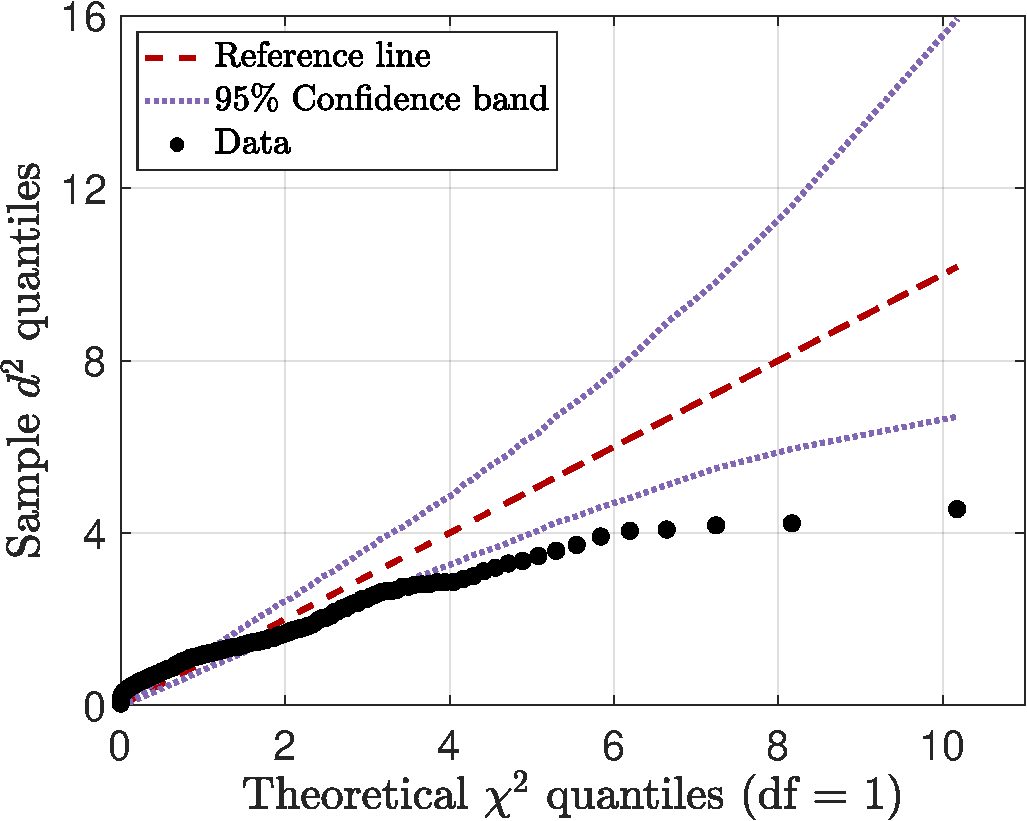
\includegraphics[height=0.36\linewidth]{./figures/test_normal.pdf}&
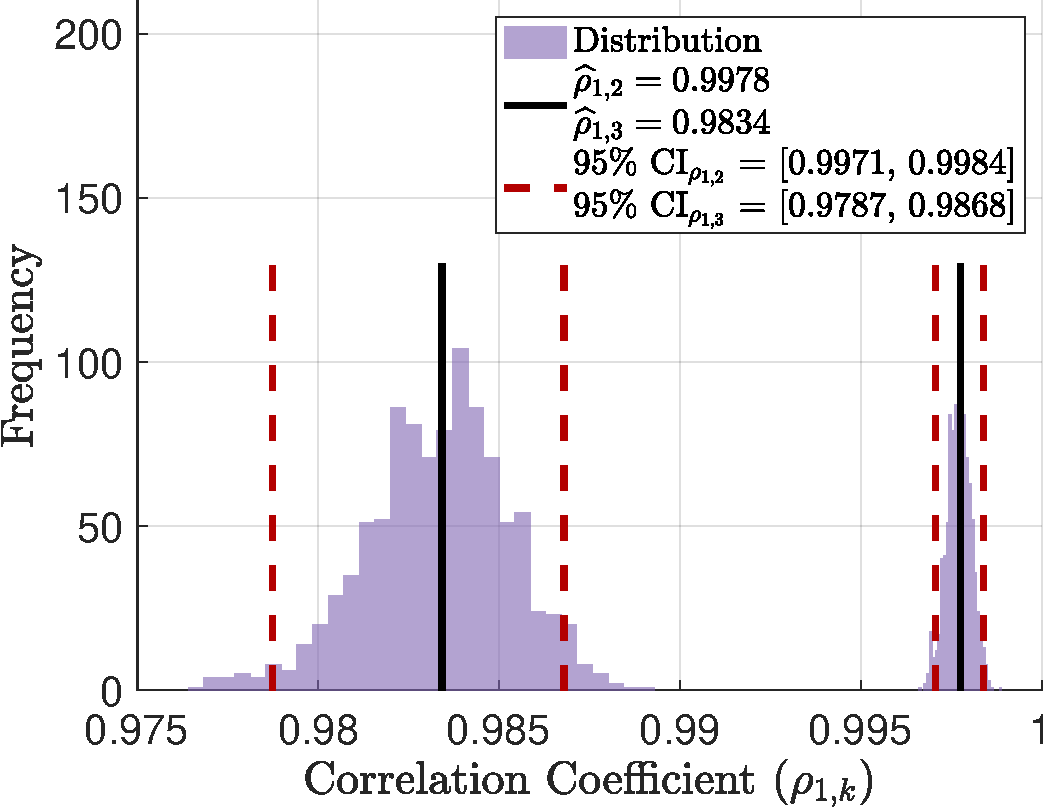
\includegraphics[height=0.36\linewidth]{./figures/CI_BCa_8e3.pdf}
\end{tabular}
\caption{Left: Quantile–quantile plot of squared Mahalanobis distances versus the $\chi^2(1)$ distribution with one degree of freedom, computed from 400 samples on the reference mesh. Dashed lines indicate 95\% bootstrap confidence bands based on 1000 resamples. Right: BCa confidence intervals for the correlation coefficient for $\epsilon=[6,8]\times 10^{-3}$, estimated from 50 samples with 1000 bootstrap resamples.}
\label{fig:Test_normal}
\end{figure}
%


% %
% \begin{table}[ht]
% \centering
% \scalebox{0.8}{
% \begin{tabular}{|c|c|c|c|c|c|c|c|c|c|c|c|c|c|c|c|c|c|c|}
% \cline{1-8}	
% \multirow{2}{*}{$\epsilon$}&\multicolumn{1}{|c|}{$\ell$} &0&1&2&3&4&5\\
% \cline{2-8}	
% &\multicolumn{1}{|c|}{$M_\ell$} &$2685$ &$8019$ &$30449$ &$120697$ &$484080$ &$1934365$\\
% \hline
% \multirow{2}{*}{$6\times 10^{-3}\;\;\sim \;\;8\times 10^{-3}$} &\multicolumn{1}{|c|}{Candidate model $k$} &$\widehat u_{h,3}$&$\widehat u_{h,2}$&$\widehat u_{h,1}$&\multirow{3}{*}{}&\multirow{3}{*}{}&\multirow{3}{*}{}\\
% % \cline{2-5}		
% % &\multicolumn{1}{|c|}{$\sigma_{k}$}&9.5720e-03   &1.1549e-02   &1.0939e-02&&&\\
% % \cline{2-5}	
% % &\multicolumn{1}{|c|}{$\text{Cov}\left(\widehat u_{h,1},\widehat u_{h,k}\right)$}&1.0286e-04&1.2604e-04&-&&&\\
% \cline{2-5}
% &\multicolumn{1}{|c|}{$\rho_{1,k}$}&9.8238e-01&9.9762e-01&-&&&\\
% % \hline
% % &\multicolumn{1}{|c|}{$\xi$}&8.8504e-03\\
% \hline
% \multirow{2}{*}{$2\times 10^{-3}\;\;\sim \;\;4\times 10^{-3}$} &\multicolumn{1}{|c|}{Candidate model $k$} &$\widehat u_{h,4}$&$\widehat u_{h,3}$&$\widehat u_{h,2}$&$\widehat u_{h,1}$&\multirow{3}{*}{}&\multirow{3}{*}{}\\
% % \cline{2-6}	
% % &\multicolumn{1}{|c|}{$\sigma_{k}$}&9.5720e-03   &1.1549e-02   &1.1001e-02   &1.0836e-02 &&\\
% % \cline{2-6}	
% % &\multicolumn{1}{|c|}{$\text{Cov}\left(\widehat u_{h,1},\widehat u_{h,k}\right)$} &1.0206e-04 &1.2480e-04 &1.1911e-04 &- &&\\
% \cline{2-6}	
% &\multicolumn{1}{|c|}{$\rho_{1,k}$}&9.8394e-01&9.9720e-01 &9.9919e-01&-&&\\
% % \hline
% % &\multicolumn{1}{|c|}{$\xi$}&2.7609e-03\\
% \hline
% \multirow{2}{*}{$4\times 10^{-4}\;\;\sim \;\;1\times 10^{-3}$} &\multicolumn{1}{|c|}{Candidate model $k$} &$\widehat u_{h,5}$&$\widehat u_{h,4}$&$\widehat u_{h,3}$&$\widehat u_{h,2}$&$\widehat u_{h,1}$&\multirow{3}{*}{}\\
% %  \cline{2-7}	
% % &\multicolumn{1}{|c|}{$\sigma_{k}$}&9.5720e-03   &1.1549e-02   &1.1001e-02   &1.0838e-02   &1.0840e-02  &\\
% % \cline{2-7}	
% % &\multicolumn{1}{|c|}{$\text{Cov}\left(\widehat u_{h,1},\widehat u_{h,k}\right)$}&1.0209e-04 &1.2485e-04 &1.1916e-04 &1.1745e-04 &- &\\
% \cline{2-7}	
% &\multicolumn{1}{|c|}{$\rho_{1,k}$}&9.8392e-01 &9.9727e-01 &9.9925e-01 &9.9977e-01 &- &\\
% % \hline
% % &\multicolumn{1}{|c|}{$\xi$}&7.7012e-04\\
% \hline
% \multirow{2}{*}{$2\times 10^{-4}$} &\multicolumn{1}{|c|}{Candidate model $k$} &$\widehat u_{h,6}$&$\widehat u_{h,5}$&$\widehat u_{h,4}$&$\widehat u_{h,3}$&$\widehat u_{h,2}$&$\widehat u_{h,1}$\\
% % \cline{2-8}
% % &\multicolumn{1}{|c|}{$\sigma_{k}$}&9.5720e-03   &1.1549e-02   &1.1001e-02   &1.0838e-02   &1.0812e-02  &1.0840e-02\\
% % \cline{2-8}	
% % &\multicolumn{1}{|c|}{$\text{Cov}\left(\widehat u_{h,1},\widehat u_{h,k}\right)$}&1.0209e-04&1.2485e-04&1.1916e-04&1.1745e-04&1.1717e-04&-\\
% \cline{2-8}	
% &\multicolumn{1}{|c|}{$\rho_{1,k}$}&9.8390e-01   &9.9728e-01   &9.9925e-01   &9.9977e-01   &9.9976e-01   &-\\
% % \hline
% % &\multicolumn{1}{|c|}{$\xi$}&5.9298e-04\\
% \hline
% \end{tabular}}
% \caption{Estimated statistical parameters for various predetermined tolerances $\epsilon$ in terms of nMSE with 500 samples for approximating parameters between each low fidelity models and the corresponding high fidelity model. The high-fidelity model $\widehat u_{h,1}$ represents the finite element solution to the free boundary problem on a spatial grid of level $L$, ensuring the discretization error meets accuracy requirements. Candidate low-fidelity models $\widehat u_{h,k}$ for $k \geq 2$ are generated using 25 sparse grid nodes (with level $q=1$) on spatial grids from levels 0 to $L-1$. All parameters are estimated using Welford's dynamic sampling algorithm with a stopping criterion requiring a relative error of $10^{-4}$ for all parameters.}
% \label{Tab:MFMC_parameters}
% \end{table}
% %



% %
% \begin{table}[ht]
% \centering
% \scalebox{0.8}{
% \begin{tabular}{c|c|c|c|c|c|c|c|c|c|c|c|c|c|c|c|c|c|c|}
% \cline{1-7}	
% \multicolumn{1}{|c|}{$\ell$} &0&1&2&3&4&5\\
% \hline
% \multicolumn{1}{|c|}{$M_\ell$} &$2685$ &$8019$ &$30449$ &$120697$ &$484080$ &$1934365$\\
% % \hline
% % \multicolumn{1}{|c|}{Model $k$} &$f_1$&$f_2$&$f_3$&$f_4$&$f_5$&$f_6$\\
% \hline
% \multicolumn{1}{|c|}{$W_\ell$ direct solve}&4.88e-02 &1.49e-01 &6.33e-01 &3.23e+00 &1.55e+01 &7.30e+01\\
% \hline
% \multicolumn{1}{|c|}{$W_\ell^e$ surrog evaluation}&2.68e-04   &5.06e-04   &1.40e-03   &7.03e-03   &2.17e-02   &9.71e-02\\
% \hline
% % \multicolumn{1}{|c|}{$C_\ell$ surrog evaluation( nodes)-source term}&\\
% % \hline
% \end{tabular}}
% \caption{The number of spatial grid points $M_\ell$, cost per sample for both direct computation $W_\ell$ and surrogate evaluation $W_\ell^e$ at an increasing spatial grid level $\ell = 0$ to 5.}
% % and surrogate evaluation with level $q=1$ sparse grid nodes ($P=$)  in the source term.}
% \label{Tab:Dof}
% \end{table}
% %

%
\begin{figure}[ht!]\centering
\begin{tabular}{cc}
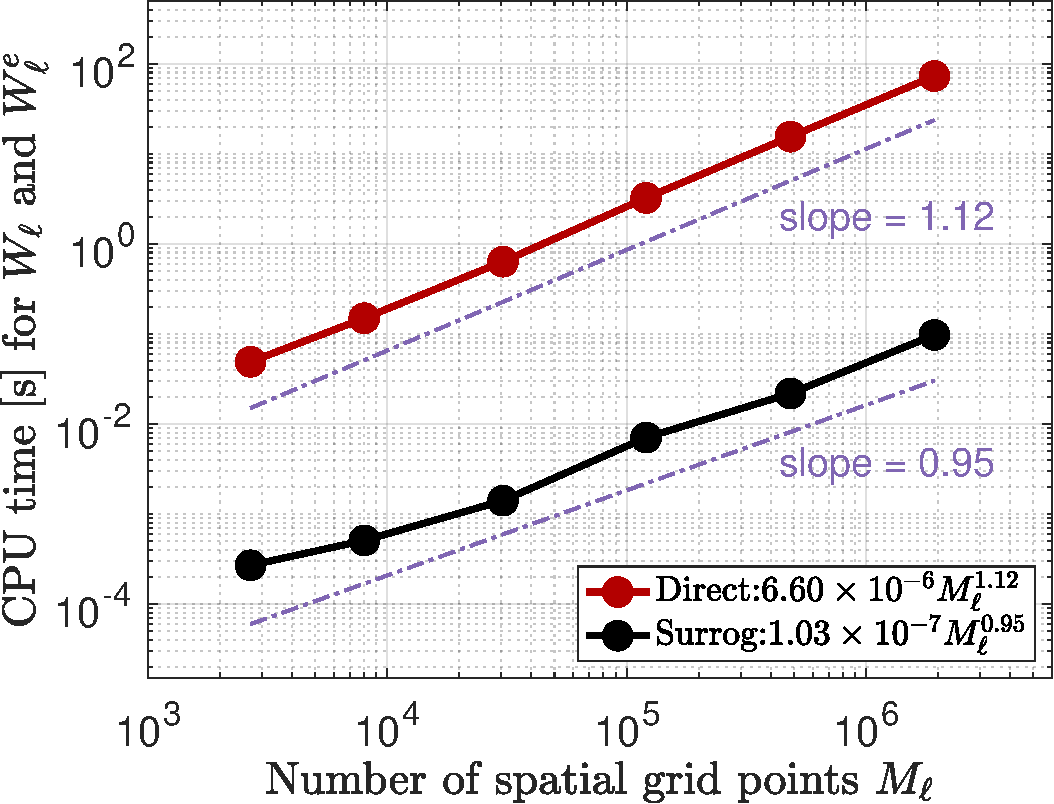
\includegraphics[height=0.36\linewidth]{./figures/CostPerSample_Ml.pdf}&
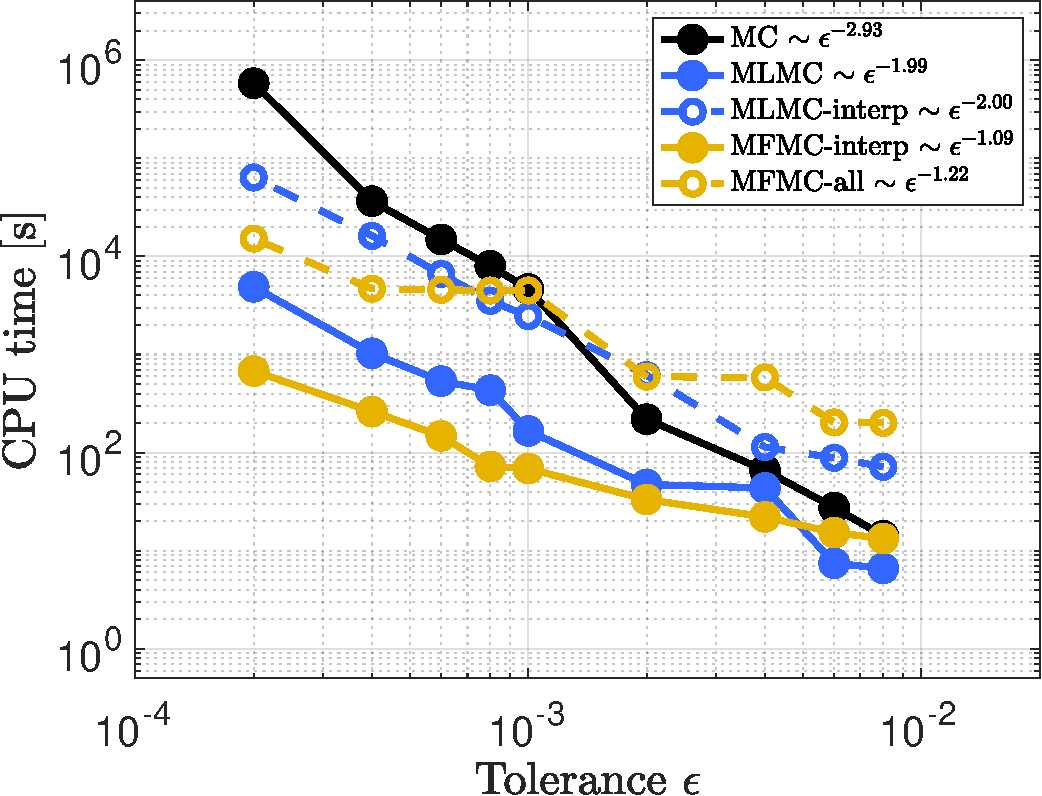
\includegraphics[height=0.36\linewidth]{./figures/Cost_epsilon.pdf}
\end{tabular}
\caption{Left: Mean CPU times of 500 realizations for direct computations $W_\ell$ and surrogate evaluations $W_\ell^e$ versus the number of spatial grid points $M_\ell$ for $\ell = 0$ to 5. Right: Total CPU time versus $\epsilon$ for different simulation methods.}
\label{fig:CostEstimatePlot}
\end{figure}
%




 
 % While the offline preparation incurs non-negligible computational expenses, these costs are justified by the substantial savings achieved during large-scale online sampling, particularly in applications requiring thousands of high-fidelity model evaluations. As a one-time expense, the precomputed surrogates and statistical parameters are reused throughout the online phase, amortizing the initial overhead across all subsequent multi-fidelity Monte Carlo realizations.







% %
% \begin{table}[ht]
% \centering
% \scalebox{0.8}{
% \begin{tabular}{c|c|c|c|c|c|c|c|c|c|c|c|c|c|c|c|c|c|c|}
% \cline{1-7}	
% \multicolumn{1}{|c|}{$\ell$} &0&1&2&3&4&5\\
% \hline
% \multicolumn{1}{|c|}{$M_\ell$} &$2685$ &$8019$ &$30449$ &$120697$ &$484080$ &$1934365$\\
% \hline
% \multicolumn{1}{|c|}{Model $k$} &$\widehat u_{h,5}$&$\widehat u_{h,4}$&$\widehat u_{h,3}$&$\widehat u_{h,2}$&&\\
% \hline
% \multicolumn{1}{|c|}{$\rho_{1,k}$ (24 nodes), ref l=3}&0.9802&0.9958 &0.9976&0.9984&&\\
% \hline
% \multicolumn{1}{|c|}{$\sigma_{k}$}&9.3826e-05 &1.374e-04 &1.2405e-04 &1.2016e-04 &&\\
% \hline
% \multicolumn{1}{|c|}{Covariance} &1.0807e-04 &1.3283e-04 &1.2646e-04 &1.2457e-04 &&\\
% \hline
% \end{tabular}}
% \caption{$\epsilon = 4\times 10^{-3}\;\;\& \;\;2\times 10^{-3}$. High fidelity model: finite element solution on mesh with 120697 grid nodes. $\sigma_1 = 1.2955e-04$. The data are estimated using 500 samples. The selected models are $[\widehat u_{h,2},\widehat u_{h,4},\widehat u_{h,5}]$.}
% % \label{Tab:Dof}
% \end{table}
% %

% %
% \begin{table}[ht]
% \centering
% \scalebox{0.8}{
% \begin{tabular}{c|c|c|c|c|c|c|c|c|c|c|c|c|c|c|c|c|c|c|}
% \cline{1-7}	
% \multicolumn{1}{|c|}{$\ell$} &0&1&2&3&4&5\\
% \hline
% \multicolumn{1}{|c|}{$M_\ell$} &$2685$ &$8019$ &$30449$ &$120697$ &$484080$ &$1934365$\\
% \hline
% \multicolumn{1}{|c|}{Model $k$} &$\widehat u_{h,6}$&$\widehat u_{h,5}$&$\widehat u_{h,4}$&$\widehat u_{h,3}$&$\widehat u_{h,2}$&\\
% \hline
% \multicolumn{1}{|c|}{$\rho_{1,k}$ (24 nodes), ref l=3}&9.0103e-01 &9.2531e-01 &9.2415e-01 &9.2366e-01 &9.2307e-01 &\\
% \hline
% \multicolumn{1}{|c|}{$\sigma_{k}$}&1.1064e-04 &1.3571e-04 &1.2930e-04 &1.2757e-04  &1.2742e-04  &\\
% \hline
% \multicolumn{1}{|c|}{Covariance}&8.9789e-05 &1.2808e-04 &1.1657e-04 &1.1358e-04 &1.1346e-04 &\\
% \hline
% \end{tabular}}
% \caption{$\epsilon = 1\times 10^{-3}\;\;\& \;\;8\times 10^{-4}\;\;\& \;\;6\times 10^{-4}\;\;\& \;\;4\times 10^{-4}$. High fidelity model: finite element solution on mesh with 484080 grid nodes. $\sigma_1 = 1.6794e-04$. The data are estimated using 500 samples.}
% % \label{Tab:Dof}
% \end{table}
% %





% =============================
\subsection{Sampling (online) cost} \label{sec:Online_Sampling}
% =============================
We now perform online sampling  to compute the MFMC estimator using the parameters $\widehat\rho_{1,k}$ and $\widehat \alpha_k$ estimated offline by Algorithm~\ref{algo:Parameter_Estimation}.  Given the prohibitively expensive cost of evaluating the high-fidelity model, one might be tempted to reuse samples from the offline phase during online estimation. However, such sample reuse compromises the statistical independence required for unbiasedness. Specifically, the control variate weights $\widehat\alpha_k$ become random variables dependent on the same realizations used to compute $Y_k$, which induces statistical dependence. As a result, the key identity $\mathbb{E}[\widehat\alpha_k Y_k] = \widehat\alpha_k \mathbb{E}[Y_k]=0$ for $k\ge 2$ no longer holds. Instead, $\mathbb{E}[\widehat\alpha_k Y_k] = \mathbb{E}[\widehat\alpha_k Y_k]-\mathbb{E}[\widehat\alpha_k]\mathbb{E}[Y_k] = \text{Cov}[\widehat\alpha_k,Y_k]\neq 0$, which leads to a biased estimator, $\mathbb{E}[A^{\text{MF}}] \neq \mathbb{E}[Y_1]$. Therefore, to preserve unbiasedness, it is essential to maintain disjoint sample sets between the offline parameter estimation and the online estimator construction. Although \cite{KoFaPeDiJeNeBu:2022} observes that the resulting bias may be negligible in practice, this observation does not eliminate the need for rigorous statistical independence. In contrast, MLMC is structurally immune to this issue due to its fixed weights $\alpha_k \equiv 1$, which allow full sample reuse without introducing bias.


The right panel of Figure~\ref{fig:CostEstimatePlot} shows the online sampling costs for various methods over a range of tolerances $\epsilon$. For our MFMC and MLMC, which rely on non-nested geometry-conforming discretizations and, therefore, incompatible mesh domains, all correction terms in the estimator for \eqref{eq:QoI} are interpolated onto a common fine grid prior to aggregation to mitigate extrapolation errors. For each sample, MLMC solutions at different levels are interpolated to a common reference grid at level $\ell=5$, while MFMC corrections -- computed via stochastic collocation using coarse finite element discretizations -- are interpolated only during the construction of the low-fidelity surrogates in the offline stage. This approach requires no additional interpolation during sample evaluation. The results show that for moderate tolerances $\epsilon > 10^{-3}$, MFMC incurs higher total cost than both MC and MLMC, mainly due to the offline overhead associated with the construction of low-fidelity models and parameter estimation. However, as $\epsilon$ decreases, the asymptotic efficiency of MFMC becomes apparent. Below $\epsilon = 10^{-3}$, MFMC outperforms both alternatives in total cost.

To interpret these empirical trends, we compare the observed sampling costs with theoretical predictions derived from asymptotic cost theorems. Implementation details for both MC and MLMC are provided in \cite{ElLiSa:2023}.  For standard Monte Carlo, the cost scales as $\epsilon^{-2 - \gamma/\alpha} \approx \epsilon^{-3.1}$, consistent with the observed rate $\epsilon^{-2.93}$. MLMC exhibits the optimal theoretical rate $\epsilon^{-2}$,  in close agreement with the measured rate $\epsilon^{-1.99}$. 

For MFMC, the asymptotic cost is governed by \eqref{eq:MFMC_sampling_cost}, as established in Theorem~\ref{thm:Sample_cost_est}. A key observation in our setting is that the high-fidelity model dominates the overall computational budget. For instance, at tolerance $\epsilon = 2 \times 10^{-4}$, we find that the leading term $\sqrt{C_1 \Delta_1} \approx 0.191$ significantly outweighs the aggregate contribution from all low-fidelity models, given by $\sum_{k=2}^{K} \sqrt{C_k \Delta_k} \approx 0.0239$. The latter is nearly an order of magnitude smaller, indicating that the cost is effectively dictated by the high-fidelity component alone. This separation of scales simplifies the asymptotic cost analysis: by Theorem~\ref{thm:Sample_cost_est}, the dominant term $\sqrt{C_1 \Delta_1}$ determines the leading-order behavior, and the total MFMC cost follows the scaling $\epsilon^{-2 + (\beta - \gamma)/\alpha}$. To evaluate this rate, we note that the second model $u_{h,2}$ -- a direct nonlinear solve on a coarser grid -- is highly correlated with the high-fidelity model, with $\rho_{1,2} \approx 1$. Under this strong correlation, Lemma~2 in \cite{PeGuWi:2018} implies that the MFMC variance decay rate $\beta$ coincides with that of MLMC. Based on empirical evidence in \cite{ElLiSa:2023}, we adopt $\beta \approx 2$, and take $\alpha \approx 1$ from \cite{ElLiSa:2023, ElLiSa:2025}. The cost growth rate $\gamma \approx 1.1$ is extracted from Figure\ref{fig:CostEstimatePlot}. Substituting into the asymptotic formula yields the rate $\epsilon^{-2 + (2 - 1.1)/1} = \epsilon^{-1.09}$, which aligns with the observed MFMC scaling. These results confirm consistency between the theoretical predictions and empirical sampling performance across all methods.


Table~\ref{Tab:CPU_time} presents the empirical CPU time and corresponding speed-ups for various simulation methods, benchmarked against standard Monte Carlo, across a range of error tolerances. At a target tolerance of $\epsilon = 2\times 10^{-4}$, the multifidelity Monte Carlo method with interpolation (MFMC-FE(Interp)) achieves a remarkable $38.4$ speedup, significantly outperforming the multilevel Monte Carlo, which attains only $9.2$. This substantial performance gap underscores the superior asymptotic scaling behavior of MFMC when equipped with an interpolated model hierarchy. The observed deviations from the theoretical speedups predicted by~\eqref{eq:MFMC_sampling_cost_efficiency} are largely due to the interpolation overhead, which is especially pronounced at higher tolerances where fixed computational costs constitute a non-negligible portion of total runtime. As expected, incorporating offline costs reduces efficiency for moderate tolerances; however, this effect becomes negligible once $\epsilon \leq 10^{-3}$, where online sampling dominate the total cost.
%
\begin{table}[ht]
	\centering
			\scalebox{0.9}{
   \begin{tabular}{c|c|c|c|c|c|c|c|c|c|c|c|c|}
			\hline
			\multicolumn{1}{|c|}{ }&MC-FE &MLMC-FE&MLMC-FE(Interp)
            % &MFMC-FE 
            &MFMC-FE(Interp)&MFMC-FE(Interp)+offline\\
			\multicolumn{1}{|c|}{$\epsilon$}&Time &\begin{tabular}{cc} \,\,\,\,\,Time & \,\,\,Speedup \end{tabular}&\begin{tabular}{cc} \,\,\,\,Time & \,\,\,Speedup \end{tabular} &\begin{tabular}{cc} \,\,\,\,Time & \,\,\,Speedup \end{tabular} &\begin{tabular}{cc} \,\,\,\,Time & \,\,\,Speedup \end{tabular}\\
            % &\begin{tabular}{cc} \,\,\,\,Time & \,\,\,Speedup \end{tabular}\\
			\hline
			\multicolumn{1}{|c|}{$8\times 10^{-3} $}&1.42e+01&\begin{tabular}{cc}6.61e+00\,\,\, & 2.1 \end{tabular}&\begin{tabular}{cc}7.17e+01\,\,  &0.2\end{tabular}
            % &\begin{tabular}{cc}7.2998e+00\,\,  &1.9453e+00 \end{tabular} 
            &\begin{tabular}{cc}1.33e+01\,\,   &1.1 \end{tabular} &\begin{tabular}{cc}2.01e+02\,\,  &0.07\end{tabular}\\
			\multicolumn{1}{|c|}{$6\times 10^{-3} $}&2.75e+01&\begin{tabular}{cc}7.44e+00\,\,\, & 3.7 \end{tabular}&\begin{tabular}{cc}8.84e+01\,\,  &0.3\end{tabular}
            % &\begin{tabular}{cc}9.3266e+00\,\, &2.9486e+00 \end{tabular}
            &\begin{tabular}{cc}1.53e+01&1.8
            \end{tabular}&\begin{tabular}{cc}2.03e+02\,\,  &0.1\end{tabular}\\
			\multicolumn{1}{|c|}{$4\times 10^{-3} $}&6.60e+01&\begin{tabular}{cc}4.36e+01\,\,\, & 1.5 \end{tabular}&\begin{tabular}{cc}1.14e+02\,\,  &0.6\end{tabular}
            % &\begin{tabular}{cc}1.9119e+01&3.4521e+00\end{tabular}
            &\begin{tabular}{cc}2.21e+01&3.0
            \end{tabular}&\begin{tabular}{cc}5.84e+02\,\,  &0.1\end{tabular}\\
			\multicolumn{1}{|c|}{$2\times 10^{-3} $}&2.19e+02&\begin{tabular}{cc}4.73e+01\,\, & 4.6\end{tabular}&\begin{tabular}{cc}6.16e+02\,\,  &0.4\end{tabular}
            % &\begin{tabular}{cc}3.0242e+01& 7.2416e+00\end{tabular}
            &\begin{tabular}{cc}3.32e+01&6.6 \end{tabular}&\begin{tabular}{cc}5.95e+02\,\,  &0.4\end{tabular}\\
			\multicolumn{1}{|c|}{$10^{-3} $}&4.66e+03&\begin{tabular}{cr}1.66e+02\,\, & 28.1 \end{tabular}&\begin{tabular}{cc}2.46e+03\,\,  &1.9\end{tabular}
            % &\begin{tabular}{cc}6.5732e+01&7.0894e+01\end{tabular}
            &\begin{tabular}{cc}6.87e+01&67.9
            \end{tabular}&\begin{tabular}{cc}4.49e+03\,\,  &1.0\end{tabular}\\
			\multicolumn{1}{|c|}{$8\times 10^{-4} $}&8.02e+03&\begin{tabular}{cc}4.33e+02\,\, & 18.5 \end{tabular}&\begin{tabular}{cc}3.53e+03\,\,  &2.3\end{tabular}
            % &\begin{tabular}{cc}6.9345e+01&1.1565e+02\end{tabular}
            &\begin{tabular}{cc}7.23e+01&111.0
            \end{tabular}&\begin{tabular}{cc}4.49e+03\,\,  &1.8\end{tabular}\\
			\multicolumn{1}{|c|}{$6\times 10^{-4} $}&1.49e+04&\begin{tabular}{cc}5.36e+02\,\, & 27.8 \end{tabular}&\begin{tabular}{cc}6.63e+03\,\,  &2.2\end{tabular}
            % &\begin{tabular}{cc}1.4482e+02&1.0289e+02\end{tabular}
            &\begin{tabular}{cc}1.48e+02&100.6
            \end{tabular}&\begin{tabular}{cc}4.57e+03\,\,  &3.3\end{tabular}\\
                \multicolumn{1}{|c|}{$4\times 10^{-4} $}&3.66e+04&\begin{tabular}{cc}1.03e+03\,\, & 35.4 \end{tabular}&\begin{tabular}{cc}1.62e+04\,\,  &2.3\end{tabular} &\begin{tabular}{cc}2.62e+02&139.7 \end{tabular}
                % &\begin{tabular}{cc}2.6595e+02&1.3762e+02\end{tabular}
            &\begin{tabular}{cc}4.68e+03\,\,  &7.8\end{tabular}\\
                \multicolumn{1}{|c|}{$2\times 10^{-4} $}&5.84e+05$^{\ast}$\!\!\!&\begin{tabular}{cc}4.90e+03 &119.2 \end{tabular} &\begin{tabular}{cc}6.38e+04\,\,  &9.2\end{tabular}
                % &\begin{tabular}{cc} 6.6985e+02&8.7184e+02 \end{tabular}
                &\begin{tabular}{cc}6.78e+02 &861.2 \end{tabular}&\begin{tabular}{cc}1.52e+04\,\,  &38.4\end{tabular}\\
			\hline
	\end{tabular}
 }
	\caption{CPU time (seconds) and speedup relative to MC-FE at various tolerances $\epsilon$. Methods include Monte Carlo (MC-FE), multilevel Monte Carlo (MLMC-FE), MLMC with interpolation to a common grid at level $\ell=5$ (MLMC-FE(Interp)), multifidelity Monte Carlo with interpolation (MFMC-FE(Interp)), and MFMC including offline costs. The asterisk indicates an estimated MC-FE time due to prohibitive computational cost.}
	\label{Tab:CPU_time}
\end{table}
%

The efficiency advantage of MFMC originates from its allocation of samples across fidelity levels, as detailed in Table~\ref{Tab:SampleSize}. As the target tolerance decreases, all methods naturally increase their total sample counts and use finer discretizations. However, MFMC dramatically shifts the sampling effort toward low-fidelity models, resulting in an efficient trade-off between variance reduction and cost. At $\epsilon = 2\times 10^{-4}$, MFMC assigns 97,028 samples to level $\ell = 0$, compared to just 15,619 in MLMC and none in MC, accounting for 97.1\% low-fidelity usage for MFMC versus 93.8\% for MLMC. While MFMC uses approximately 6.2 times more samples than MLMC overall, its emphasis on inexpensive evaluations results in a $93.6$  times reduction in online sampling cost. This sample allocation leads to substantial net gains in computational efficiency, particularly in the high-accuracy regime, where the cost of high-fidelity models becomes prohibitive.

%
\begin{table}[ht]
	\centering
			\scalebox{0.7}{
   \begin{tabular}{c|c|c|c|c|c|c|c|c|c|c|c|c|}
	    \cline{2-7}	
		&\multicolumn{6}{|c|}{ Level $\ell$}\\
			\hline
			\multicolumn{1}{|c|}{$\epsilon$}&0&1&2&3&4&5\\
			\hline
			\multicolumn{1}{|c|}{$8\times 10^{-3} $}&&&5&&&\\
			\multicolumn{1}{|c|}{$6\times 10^{-3} $}&&&9&&&\\
			\multicolumn{1}{|c|}{$4\times 10^{-3} $}&&&&21&&\\
			\multicolumn{1}{|c|}{$2\times 10^{-3} $}&&&&73&&\\
			\multicolumn{1}{|c|}{$10^{-3} $}&&&&&287&\\
			\multicolumn{1}{|c|}{$8\times 10^{-4} $}&&&&&445&\\
			\multicolumn{1}{|c|}{$6\times 10^{-4} $}&&&&&845&\\
                \multicolumn{1}{|c|}{$4\times 10^{-4} $}&&&&&2000&\\
                \multicolumn{1}{|c|}{$2\times 10^{-4} $}&&&&&& 8000$^{\ast}$\!\!\\
			\hline
	\end{tabular}
 \qquad
		\begin{tabular}{c|c|c|c|c|c|c|c|c|c|c|c|c|}
	    \cline{2-7}	
		&\multicolumn{6}{|c|}{ Level $\ell$}\\
			\hline
			\multicolumn{1}{|c|}{$\epsilon$}&0&1&2&3&4&5\\
			\hline
			\multicolumn{1}{|c|}{$8\times 10^{-3} $}&10     &2     &2&&&\\
			\multicolumn{1}{|c|}{$6\times 10^{-3} $}&12     &2     &2&&&\\
			\multicolumn{1}{|c|}{$4\times 10^{-3} $}&22     &5     &2     &2&&\\
			\multicolumn{1}{|c|}{$2\times 10^{-3} $}&163    &26     &5     &2&&\\
			\multicolumn{1}{|c|}{$10^{-3} $}&577   &90    &15     &3     &2&\\
			\multicolumn{1}{|c|}{$8\times 10^{-4} $}&1036 &157 &26 &5 &2&\\
			\multicolumn{1}{|c|}{$6\times 10^{-4} $}&1744 &266 &44 &9 &2&\\
                \multicolumn{1}{|c|}{$4\times 10^{-4} $}&3911 &553 &86 &17 &4&\\
                \multicolumn{1}{|c|}{$2\times 10^{-4} $}&15619 &2298 &370 &57 &12 &2\\
			\hline
	\end{tabular}
 \qquad
		\begin{tabular}{c|c|c|c|c|c|c|c|c|c|c|c|c|c|c|c|c|c|}
	    \cline{2-7}	
		&\multicolumn{6}{|c|}{ Level $\ell$}\\
			\hline
			\multicolumn{1}{|c|}{$\epsilon$}&0&1&2&3&4&5\\
			\hline
			\multicolumn{1}{|c|}{$8\times 10^{-3} $}&24&4&2&&&\\
			\multicolumn{1}{|c|}{$6\times 10^{-3} $}&43&7&2&&&\\
			\multicolumn{1}{|c|}{$4\times 10^{-3} $}&95&12&4&2&&\\
			\multicolumn{1}{|c|}{$2\times 10^{-3} $}&380&46&13&2&&\\
			\multicolumn{1}{|c|}{$10^{-3} $}&2444&301&79&13&2&\\
			\multicolumn{1}{|c|}{$8\times 10^{-4} $}&3819&470&123&21&2&\\
                \multicolumn{1}{|c|}{$6\times 10^{-4} $}&6788&835&218&36&2&\\
			\multicolumn{1}{|c|}{$4\times 10^{-4} $}&15273&1879&489&81&2&\\
                \multicolumn{1}{|c|}{$2\times 10^{-4} $}&97028&13374&2544&335&-&5\\
			\hline
	\end{tabular}
 
 }
	\caption{Optimal sample size allocations for MC-FE (left), MLMC-FE (center), and MFMC-FE (right) at various error tolerances $\epsilon$. The MC entry for $\epsilon = 2 \times 10^{-4}$ (asterisk) is extrapolated due to high cost. A dash in MFMC-FE indicates the corresponding model is not selected.}    
	\label{Tab:SampleSize}
\end{table}
%




% \JLcolor{According to \cite{PeGuWi:2018}, pages A3174 and A3181–A3182, perturbations in the sample variance and sample correlation coefficients have a small impact on the overall sample size and computational work. However, from my perspective, inaccurate estimation of these statistical parameters can also affect the model selection process. If these statistics are not reliably computed, low-fidelity models with misleading characteristics may be selected or rejected incorrectly, potentially undermining the efficiency and accuracy of the MFMC framework. In particular, models that exhibit inconsistent statistical properties violating the two conditions in Theorem \ref{thm:Sample_size_est} could be included, leading to suboptimal model choices for the low-fidelity approximations and, consequently, affecting the overall performance of the multi-fidelity estimator.}






% =============================
\subsection{Properties of plasma boundary and geometric descriptors}
% =============================
Accurate identification of the plasma boundary presents a significant challenge in both MLMC and MFMC frameworks, particularly when cross-level corrections are accumulated on geometry-conforming but non-nested meshes. As established in \cite{ElLiSa:2023}, geometric distortions arise from extrapolation errors introduced by spatial resolution mismatches when projecting coarse-grid solutions onto finer discretizations. These mismatches lead to obvious topological inconsistencies near the x-point region, and degrade the fidelity of the reconstructed boundary geometry. To mitigate these artifacts and ensure geometric consistency across all estimators, we adopt an interpolation strategy, as described in Section~\ref{sec:Online_Sampling}.


The effectiveness of this strategy is demonstrated in Figure~\ref{fig:QoI_plot}, which shows near-indistinguishable plasma boundary contours across Monte Carlo, interpolated MLMC, and MFMC estimators. Quantitative validation in Table~\ref{Tab:QoI_GeoInfo} further confirms this agreement: geometric descriptors from MLMC and MFMC match the Monte Carlo reference to within 0.5\% relative error, with all key parameters agreeing to at least two decimal places. These results verify that the proposed interpolation strategy successfully maintains essential geometric features in multifidelity approximations.








%=====================================================================================
% \noindent \textbf{Plasma boundary.} 
%=====================================================================================






% %
% \begin{table}[ht]
% \centering
% \scalebox{0.8}{
% \begin{tabular}{c|c|c|c|c|c|c|c|c|c|c|c|c|c|c|c|c|c|c|}
% \cline{1-7}	
% \multicolumn{1}{|c|}{Dof} &$1934365$&$484080$&$120697$&$30449$&$8019$&$2685$\\
% \hline
% \multicolumn{1}{|c|}{Model $k$} &$f_1$&$f_2$&$f_3$&$f_4$&$f_5$&$f_6$\\
% % \hline
% % \multicolumn{1}{|c|}{$C_k$ direct solve}&1.2029e+02&2.6478e+01&5.3710e+00&1.1269e+00&2.9300e-01&9.6419e-02\\
% % \hline
% % \multicolumn{1}{|c|}{$C_k$ surrog evaluation(24 nodes)}&1.2595e-01&2.9694e-02&9.1085e-03&3.0580e-03&1.1869e-03&2.5127e-04\\
% \hline
% \multicolumn{1}{|c|}{$\rho_{1,k}$ (24 nodes), ref l=3}&&&&0.9678&0.9670&0.9488\\
% \hline
% \multicolumn{1}{|c|}{$\sigma_{k}$}&&&&1.1696e-04&1.2929e-04&8.8977e-05\\
% \hline
% \multicolumn{1}{|c|}{Covariance}&&&&1.3065e-04&1.3726e-04&1.1172e-04\\
% \hline
% \end{tabular}}
% \caption{High fidelity model: finite element solution on mesh with 30449 grid nodes. $\sigma_1 = 1.5582e-04$. The data are estimated using 500 samples.}
% % \label{Tab:Dof}
% \end{table}
% %


\begin{figure}[ht!]\centering
\scalebox{.935}{\begin{tabular}{cccc}
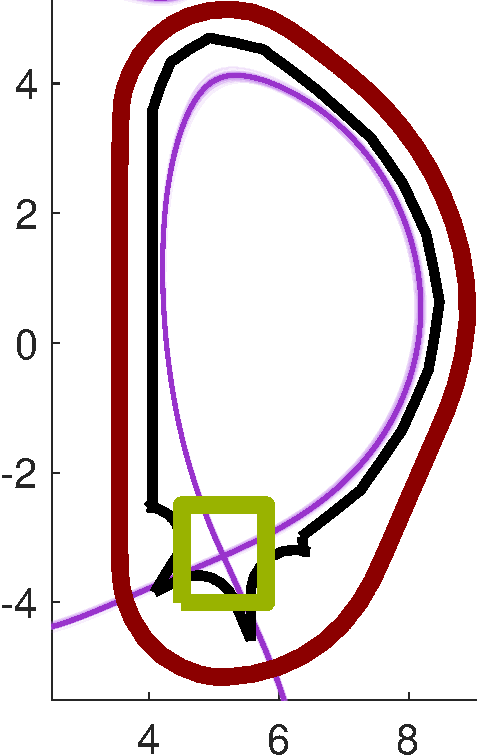
\includegraphics[width=0.19\linewidth]{./figures/Boundary_Reference.pdf} 
& 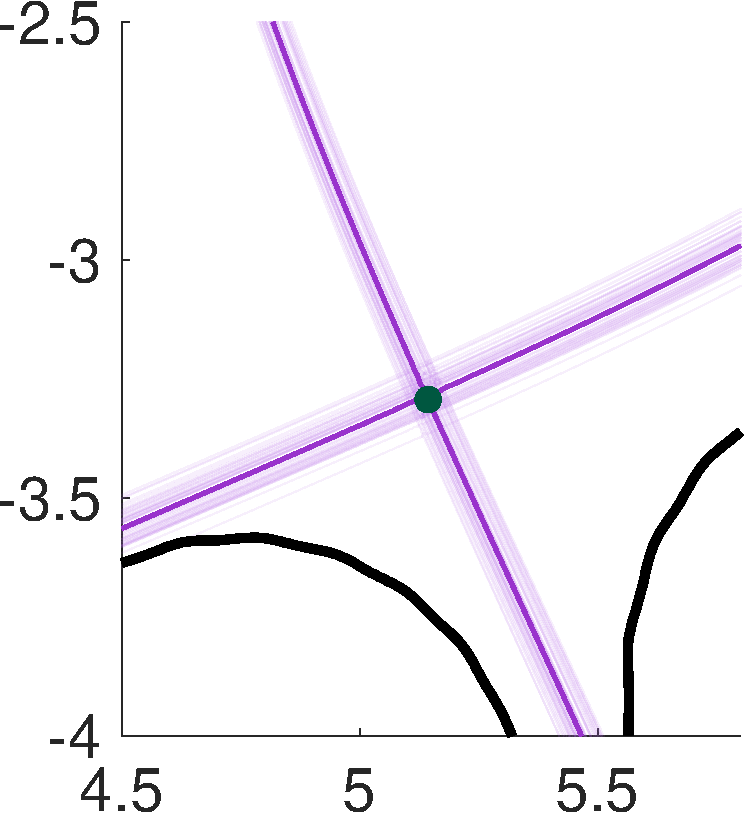
\includegraphics[width=0.19\linewidth]{./figures/QoI_MC_uniform_xptRegion.pdf} 
&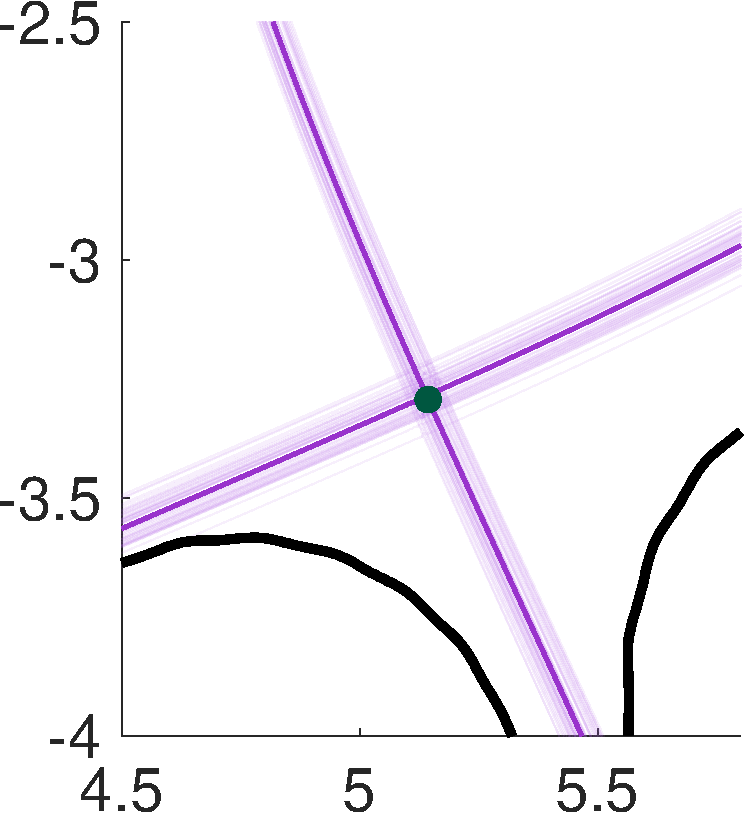
\includegraphics[width=0.19\linewidth]{./figures/QoI_MLMC_DirectSolver_xptRegion_Interp2CommonGrid.pdf}
&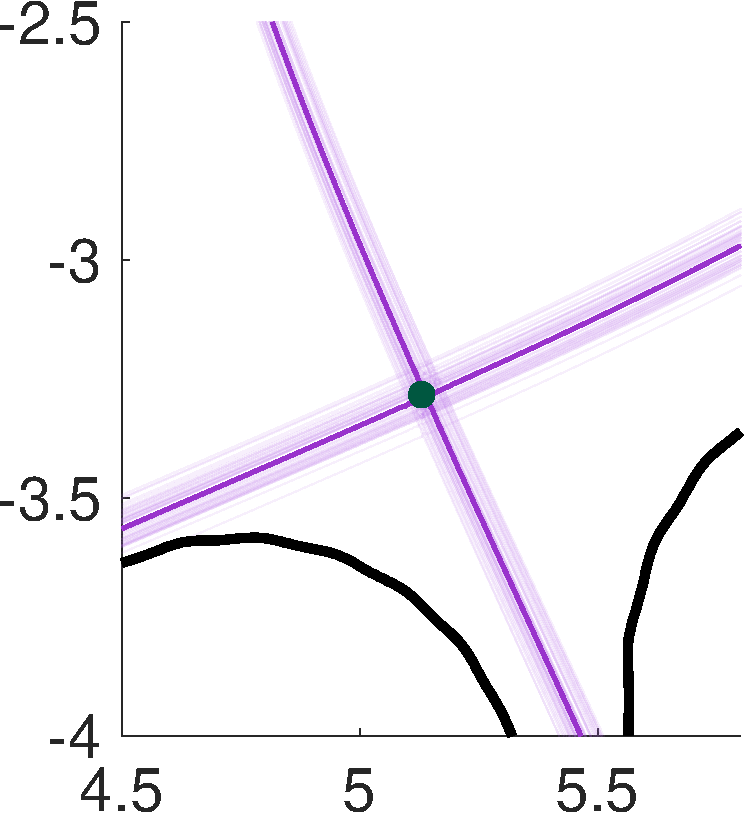
\includegraphics[width=0.19\linewidth]{./figures/QoI_MFMC_xptRegion.pdf}
\\[1ex]
Reactor & MC-FE &MLMC-FE (Interp) &MFMC-FE (Interp) \\[-0.5ex]
\end{tabular}}
\caption{The plasma boundaries of 50 random realizations are overlaid in the top row as violet curves. The solid violet line represents the plasma boundary of the expected poloidal flux generated with tolerance $\epsilon=4\times 10^{-4}$. The reactor's inner and outer walls are shown in solid black and dark red, respectively. The bottom row provides a detailed view of the regions close to the x-points, with dark green dots indicating the x-points of the expected solution. The columns, from left to right, show the simulations using the MC-FE, MLMC-FE, and MFMC-FE approaches, all interpolated to geometry-conforming uniform meshes at discretization level $\ell=5$.}
\label{fig:QoI_plot}
\end{figure}












% \noindent \textbf{Geometric descriptors.}
%
\begin{table}[ht]
	\centering
			\scalebox{0.9}{
		\begin{tabular}{c|c|c|c|c|c|c|}
			\cline{2-5}
				&\multicolumn{1}{c|}{MC-FE}&MLMC-FE&MLMC-FE (Interp)&MFMC-FE (Interp)\\
			\hline
			\multicolumn{1}{|c|}{x point}&(5.14,-3.29)&(5.14,-3.29)&(5.14,-3.29)&(5.14,-3.29)\\
			\hline
			\multicolumn{1}{|c|}{magnetic axis}&(6.41,0.61)&(6.44,0.56)&(6.41,0.61)&(6.41,0.61)\\
			\hline
			\multicolumn{1}{|c|}{strike} &(4.16,-3.71)&(4.16,-3.71)&(4.16,-3.71)&(4.16,-3.71)\\
			\multicolumn{1}{|c|}{points}&(5.56,-4.22)&(5.56,-4.22)&(5.56,-4.22)&(5.56,-4.22)\\
			\hline
			\multicolumn{1}{|c|}{inverse aspect ratio} &0.32&0.32&0.32&0.32\\
			\hline
			\multicolumn{1}{|c|}{elongation} &1.86&1.87&1.86&1.86\\
			\hline
			\multicolumn{1}{|c|}{upper triangularity}&0.43&0.43&0.43&0.43\\
			\hline
			\multicolumn{1}{|c|}{lower triangularity} &0.53&0.53&0.53&0.53\\
			\hline
	\end{tabular}
  }
	\caption{Geometric parameters of the expected poloidal flux $u$ computed using four simulation methods: MC-FE with direct solver, MLMC-FE with direct solver, MLMC-FE with interpolation to a common fine grid at level $\ell = 5$, and MFMC-FE with interpolation to the same fine grid. All results correspond to a target nMSE of $4 \times 10^{-4}$.}
	\label{Tab:QoI_GeoInfo}
\end{table}







% % =============================
% \subsection{Uncertainties in the source term}
% % =============================
% In this experiment, we study the uncertainty in perturbing the reference parameter that characterizes the source term \eqref{eq:source}.
% \begin{table}[ht]
% 	\centering
% 			\scalebox{0.62}{
%    \begin{tabular}{c|c|c|c|c|c|c|c|c|c|c|c|c|}
% 	    \cline{2-7}	
% 		&\multicolumn{6}{|c|}{ Level $\ell$}\\
% 			\hline
% 			\multicolumn{1}{|c|}{$\epsilon$}&0&1&2&3&4&5\\
% 			\hline
% 			\multicolumn{1}{|c|}{$8\times 10^{-3} $}&&&8&&&\\
% 			\multicolumn{1}{|c|}{$6\times 10^{-3} $}&&&10&&&\\
% 			\multicolumn{1}{|c|}{$4\times 10^{-3} $}&&&&25&&\\
% 			\multicolumn{1}{|c|}{$2\times 10^{-3} $}&&&&93&&\\
% 			\multicolumn{1}{|c|}{$10^{-3} $}&&&&&423&\\
% 			\multicolumn{1}{|c|}{$8\times 10^{-4} $}&&&&&678&\\
% 			\multicolumn{1}{|c|}{$6\times 10^{-4} $}&&&&&1211&\\
%                 \multicolumn{1}{|c|}{$4\times 10^{-4} $}&&&&&2700$^{\ast}$&\\
%                 \multicolumn{1}{|c|}{$2\times 10^{-4} $}&&&&&&11000$^{\ast}$\!\!\\
% 			\hline
% 	\end{tabular}
%  \qquad
% 		\begin{tabular}{c|c|c|c|c|c|c|c|c|c|c|c|c|}
% 	    \cline{2-7}	
% 		&\multicolumn{6}{|c|}{ Level $\ell$}\\
% 			\hline
% 			\multicolumn{1}{|c|}{$\epsilon$}&0&1&2&3&4&5\\
% 			\hline
% 			\multicolumn{1}{|c|}{$8\times 10^{-3} $}&10 &2 &2&&&\\
% 			\multicolumn{1}{|c|}{$6\times 10^{-3} $}&11 &3 &2 &&&\\
% 			\multicolumn{1}{|c|}{$4\times 10^{-3} $}&33 &7 &2 &2&&\\
% 			\multicolumn{1}{|c|}{$2\times 10^{-3} $}&150 &27 &4 &2&&\\
% 			\multicolumn{1}{|c|}{$10^{-3} $}&692 &116 &19 &4 &2&\\
% 			\multicolumn{1}{|c|}{$8\times 10^{-4} $}&1008 &160 &27 &6 &2&\\
% 			\multicolumn{1}{|c|}{$6\times 10^{-4} $}&2022 &322 &53 &10 &3&\\
%                 \multicolumn{1}{|c|}{$4\times 10^{-4} $}&4158 &613 &106 &14 &4&\\
%                 \multicolumn{1}{|c|}{$2\times 10^{-4} $}&17158 &2612 &442 &59 &13 &2\\
% 			\hline
% 	\end{tabular}
%  \qquad
% 		\begin{tabular}{c|c|c|c|c|c|c|c|c|c|c|c|c|c|c|c|c|c|}
% 	    \cline{2-7}	
% 		&\multicolumn{6}{|c|}{ Level $\ell$}\\
% 			\hline
% 			\multicolumn{1}{|c|}{$\epsilon$}&0&1&2&3&4&5\\
% 			\hline
% 			\multicolumn{1}{|c|}{$8\times 10^{-3} $}&&&&&&\\
% 			\multicolumn{1}{|c|}{$6\times 10^{-3} $}&&&&&&\\
% 			\multicolumn{1}{|c|}{$4\times 10^{-3} $}&&&\\
% 			\multicolumn{1}{|c|}{$2\times 10^{-3} $}&&&\\
% 			\multicolumn{1}{|c|}{$10^{-3} $}&&&&&&\\
% 			\multicolumn{1}{|c|}{$8\times 10^{-4} $}&&&&&&\\
%                 \multicolumn{1}{|c|}{$6\times 10^{-4} $}&&&&&&\\
% 			\multicolumn{1}{|c|}{$4\times 10^{-4} $}&&&&&&\\
%                 \multicolumn{1}{|c|}{$2\times 10^{-4} $}&&&&&&\\
% 			\hline
% 	\end{tabular}
 
%  }
% 	\caption{The optimal sample size estimation for MC-FE (left), uniform MLMC-FE (middle), and MFMC-FE (right). The simulations were conducted for a variety of choices of $\epsilon$. The computational cost associated with a tolerance of $\epsilon = 2\times 10^{-4}$ for Monte Carlo was prohibitive; the entry in the table for this tolerance (with an asterisk) is an estimate.}
% 	\label{Tab:SampleSize_Source_Term}
% \end{table}

% \begin{table}[ht]
% 	\centering
% 			\scalebox{0.62}{
%    \begin{tabular}{c|c|c|c|c|c|c|c|c|c|c|c|c|}
% 			\hline
% 			\multicolumn{1}{|c|}{ }&MC-FE &MLMC-FE &MFMC-FE\\
% 			\multicolumn{1}{|c|}{$\epsilon$}&Time & \begin{tabular}{cc} \,\,\,\,\,Time & \,\,\,Speedup \end{tabular}  &\begin{tabular}{cc} \,\,\,\,Time & \,\,\,Speedup \end{tabular}\\
% 			\hline
% 			\multicolumn{1}{|c|}{$8\times 10^{-3} $}&9.71e+01&\begin{tabular}{cc}1.10e+01\,\,\, & 8.8 \end{tabular}&\begin{tabular}{cc}..\,\,  & .. \end{tabular} \\
% 			\multicolumn{1}{|c|}{$6\times 10^{-3} $}&1.16e+02&\begin{tabular}{cc}1.27e+01\,\,\, & 9.1 \end{tabular}&\begin{tabular}{cc}..\,\, &.. \end{tabular}\\
% 			\multicolumn{1}{|c|}{$4\times 10^{-3} $}&1.29e+02&\begin{tabular}{cc}3.39e+01\,\,\, & 3.8 \end{tabular}&\begin{tabular}{cc}..& .. \end{tabular}\\
% 			\multicolumn{1}{|c|}{$2\times 10^{-3} $}&8.03e+02&\begin{tabular}{cc}7.29e+01\,\, & 11.0\end{tabular}&\begin{tabular}{cc}..& .. \end{tabular}\\
% 			\multicolumn{1}{|c|}{$10^{-3} $}&1.49e+04&\begin{tabular}{cr}2.55e+02\,\, & 58.5 \end{tabular}&\begin{tabular}{cc}..& .. \end{tabular}\\
% 			\multicolumn{1}{|c|}{$8\times 10^{-4} $}&3.89e+04&\begin{tabular}{cc}2.76e+02\,\, &140.6 \end{tabular}&\begin{tabular}{cc}..& ..
%             \end{tabular}\\
% 			\multicolumn{1}{|c|}{$6\times 10^{-4} $}&1.1219e+05&\begin{tabular}{cc}7.1946e+02\,\, & .. \end{tabular}&\begin{tabular}{cc}.. & .. \end{tabular}\\
%                 \multicolumn{1}{|c|}{$4\times 10^{-4} $}&..&\begin{tabular}{cc}1.1598e+03\,\, & .. \end{tabular} &\begin{tabular}{cc}..& .. \end{tabular}\\
%                 \multicolumn{1}{|c|}{$2\times 10^{-4} $}&..$^{\ast}$\!\!\!&\begin{tabular}{cc}4.4956e+03 &.. \end{tabular} &\begin{tabular}{cc}..&.. \end{tabular}\\
% 			\hline
% 	\end{tabular}
%  }
% 	\caption{The CPU time in seconds for MC-FE (left), uniform MLMC-FE (middle), and MFMC-FE (right), together with speedups for the multilevel methods, for a variety of choices of $\epsilon$. The computational cost associated with a tolerance of $\epsilon = 2\times 10^{-4}$ for Monte Carlo was prohibitive; the entry in the table for this tolerance (with an asterisk) is an estimate.}
% 	\label{Tab:CPU_time_Source_Term}
% \end{table}